\documentclass[12pt]{article}
\usepackage[utf8]{inputenc}
\usepackage[T1]{fontenc}
\usepackage{hyperref}
\usepackage{biblatex}
\usepackage{graphicx}
\usepackage{xcolor}
\usepackage{hyperref}
\usepackage{parskip}
\usepackage{enumitem}
\usepackage{listings}
\usepackage[toc,page]{appendix}
\usepackage[section]{placeins}

% Remove image float %
\usepackage{float}

% Cite all references %
\nocite{*}

\newcommand\todo[1]{\textcolor{red}{TODO : #1}}

\title{Mémoire}
\author{Rémy Pocquerusse}
\date{October 2017}

\addbibresource{references.bib}

\begin{document}

\maketitle

\par\hfil\null\par
\par\hfil\null\par
\par\hfil\null\par

\begin{center}
{\huge L'utilisation de l'intelligence artificielle pour la lutte contre la désinformation}
\end{center}

\clearpage

\renewcommand*\contentsname{Sommaire}

\clearpage

\tableofcontents

\clearpage

\section{Introduction générale}

Durant mon stage de Master 1, j'ai effectué une mission qui tournait autour d'une problématique simple : donner la possibilité à un utilisateur de décrire une chose et comprendre l'objet de cette chose côté machine. Plus précisément il me fallait catégoriser un texte pour pouvoir ensuite le classifier (parle t-on de science, d'écologie ?, etc.). Quelques pistes m'ont été données pour commencer mes recherches, notamment le traitement du langage naturelle avec les possibilitées liées au web sémantique. C'est en explorant les ambitions du web sémantique que je me suis aperçu des enjeux d'un web ouvert aux données. En formulant des requêtes en langue naturelle ou structurée (type SQL) il est possible de récupérer des données formatées et liées, exploitables par une machine. Avec l'enjouement pour l'intelligence artificielle qui a explosé grâce au big data \cite{sh}, la donnée est devenu précieuse. Beaucoup de problématiques de calcul et d'apprentissage tournent autour de la donnée, dans le machine learning par exemple il faut des données fiables, structurées et en grande quantité. La création de dataset prend du temps et nécessite souvent une intervention externe du fait de la quantité de données à traiter manuellement. Par exemple ClaimBuster (outil que nous présenterons plus tard), a nécessité 3 mois de travail et 226 participants pour créer un dataset viable \cite{hassan2015quest}.
\\*
Pourtant ces données sont disponibles sur le web. N'y aurait-il pas un moyen de réduire ce temps de 3 mois au temps d'une simple requête ?

C'est à une de ces problématiques que le web sémantique (dont nous détaillerons le fonctionnement plus tard) tente aujourd'hui de répondre. Le web sémantique avec l'intégration de la sémantique dans le web vise à donner du sens aux données. Le mot Socrate ne réfère plus à un simple mot mais à un nom, à une personne qui possède une date de naissance, une nationalité, etc. Chaque donnée va référer à un objet qui possède des attributs universels qui le décrivent \cite{schemaPerson}.
\\*
Le web sémantique a déjà eu un impact important sur le web mais méconnu, ce qui peut s'expliquer par le fait qu'il est souvent défini comme un outil fait par des scientifiques pour des scientifiques \cite{semantic_web_has_failed}.
\\*
Un des cas les plus important (et visible) est l'intégration de la sémantique dans le système de recherche de Google. Cela se traduit par des informations organisées à l'écran comme les infoboxes (panel situé à droite qui détaille notre recherche) ou encore des réponses directes aux recherches, exemple : \enquote{Quel est le vrai nom de molière ?} va nous afficher directement la réponse.

Le web sémantique a ouvert toutes sortes de données autour de différents thèmes : la médecine, le e-commerce, etc. La plupart des CMS permettent à leur utilisateurs de structurer leur données et de les ouvrir au reste du monde. Par exemple, le CMS Drupal permet de produire des données liées \cite{corlosquet2009produce}. Ce n'est pas négligeable quand on sait qu'il fait tourner environ 2.1\% de tous les sites de type CMS \cite{w3techs} (il est aussi possible de le faire sur la plupart des CMS). 
\\*
En médecine on peut noter \href{http://bio2rdf.org/}{Bio2RDF}, projet open source qui regroupe plus de 11 milliards de triples relatifs aux sciences de la vie et à la recherche clinique. On peut aussi citer DBPedia qui est une référence dans le domaine du web sémantique et qui s'est fixé pour but, depuis 2007, de produire des données liées avec des informations extraites de wikipédia.

Toutes ces données sont facilement maniables et interconnectables. Dans le cas présent nous allons voir comment ces données sont utilisées et pourrait être utilisées pour lutter contre la désinformation.

\todo{A revoir}

\subsection{La désinformation}

\enquote{La désinformation est un ensemble de techniques de communication visant à tromper des personnes ou l'opinion publique pour protéger des intérêts (privés ou non) et/ou d'influencer l'opinion publique.} \cite{wiki:desinformation}

La désinformation est donc un acte conscient et organisé pour nuire à un groupe de personnes. Elle peut se traduire par de la propagande, du prosélytisme ou de la manipulation sur tout type de sujet. Elle peut prendre tout type de configuration, mais prend souvent la forme d'allégations alarmantes ou révoltantes qui vont frapper le lecteur. Le but est de susciter une émotion forte pour que le lecteur s'empresse de partager l'information. Ceci sans vérifier aucune source. Un mensonge plus frappant qu'une vérité se diffusera plus vite et plus loin avec un impact plus important. On estime par exemple, que sur twitter, une fake news a 70\% de chance en plus d'être partagée qu'une autre information \cite{vosoughi2017rumor}. 
Ainsi la désinformation se traduit plus généralement par une tentative de manipulation de l'opinion publique (exemple \href{https://www.20minutes.fr/societe/2261439-20180426-video-evacuation-tolbiac-retour-naissance-fake-news}{ici}) en transmettant des informations partiellement erronée (il est plus facile de croire à un mensonge enrobé de vérité).

\todo{Différencier désinformation par de grandes organisation, états (propagande) de la désinformation économique/buzz (réseaux sociaux, usines à clic)}

\subsection{Fake news}

Sur internet quand on parle de désinformation, on parle de fake news ou fausses nouvelles. On définit une fake news comme étant une information dont le but est de tromper consciemment un lecteur. Une fake news peut donc être définie comme étant une tentative de désinformation mais qui pour la plupart visent à induire en erreur et créer du buzz autour d'un fait. Elle sont particulièrement présentent sur les réseaux sociaux et dans les usines à clics. Mais on les retrouvent aussi dans la presse spécialisé ou encore dans les médias politisés dont le but est la propagation de fausses information pour servir leurs intérêts (retouche d'image, etc.).  Mais un article faux n'est pas forcément une fake news tant qu'il n'y a pas l'intention de tromper, l'article peut avoir des fins humoristiques ou satiriques par exemple.

Une information se base sur un fait réel et donc vérifiable. Afin d'identifier une information comme étant fausse il faut pouvoir le prouver factuellement. Il est donc important de connaître l'existant (un ensemble d'informations vraies) pour pouvoir identifier une information fausse. Ici le but n'est pas de lutter contre ou éradiquer les fake news (cela reste de la liberté d'expression, dans une certaine mesure). Nous chercherons simplement à les identifier.

\todo{citer l'etude sur l'impact des fake news durant la campagne américaine (voir dans présentation ebs)}

\paragraph{Pourquoi favoriser leur détection ?} A cause de l'impact sur le monde réel que cela peut avoir. Susciter une vive émotion dans l'opinion publique est une des finalités de la fake news. Cela peut avoir des conséquences graves sur les évènements qui se déroulent (réponse par la violence, la haine). C'est un constat encore plus vrai en temps de guerre ou durant des périodes sensibles.

\subsection{Intelligence artificielle}

Le but de l'intelligence artificielle (IA) est de créer des machines intelligentes capables de comprendre leur environnement et de performer des actions leur permettant d'atteindre un but précis. Cela se traduit par l'imitation des facultés humaine comme la résolution de problèmes ou l'apprentissage.

\paragraph{Le Machine learning} fait référence a la capacité d'un système à apprendre de données formatées pour ensuite être capable de prédire quelque chose \cite{MichaelCopeland}.

\todo{A finir}

\subsection{Fake news et intelligence artificielle}

Détailler l'utilité de l'intelligence artificielle pour la détection de fakenews.

Machine learning ?

Vérification de source.

Vérification d'un fait : vérification d'une image ?


\subsection{Fact-checking}

\todo{Définition du fact checking et dérives (ex: fact checking system)}

\todo{Cela revient à demander à une machine de faire du journalisme. Parler des enjeux.}

\todo{Comment le fact checking intègre l'intelligence artificielle ?}

\todo{A voir, https://fullfact.org/automated}

\todo{A voir : http://idir.uta.edu/factwatcher/nba.php}

Le fact-checking ou vérification de faits représente l'acte de vérifier la véracité d'une assertion. Il s'agit de traiter l'information afin de démêler le vrai du faux, du partiellement vrai du partiellement faux.

Seulement les sources d'informations sont innombrables et le flux de données journalier est tel qu'il est impossible de vérifier chaque information manuellement. Que ce soit sur des blogs, les réseaux sociaux, les sites d'information, etc. filtrer l'information et la vérifier représente un temps de travail important.

\todo{Parler du fait que le fact-checking est une nouvelle forme de journalisme}

\paragraph{Initiatives contre les fake news}

Que fait-on dans le monde réel pour lutter contre les fakenews ?
Survey of initiatives against fake news : \cite{haciyakupoglu2018countering}

\todo{parler de facebook/google suite à la campagne américaine}

\paragraph{Fact-checking : les limites}

Le fact-checking est un travail qui est chronophage, en effet il faut tout d'abord trouver et identifier les faits vérifiable et dignes d'intérêt. Il y a ensuite un travail de recherche pour comprendre le fait et le vérifier en faisant attention de ne pas tomber soi-même dans le piège de la désinformation. Cela signifie confronter et vérifier ses sources. 
Tous ces critères font qu'entre le moment ou une déclaration est faite, et celui ou elle est vérifiée s'écoule un certain laps de temps, qui peut éventuellement rendre le fact-checking inutile si la déclaration a déjà eu l'impact voulu.

\paragraph{Quels objectifs ?}

L'objectif derrière le fact checking reste actuellement très politique, il s'agit de traquer les mensonges de personnalités influentes.

Mais à terme le fact checking doit permettre de toujours manipuler une information avérée et sûre quelque soit sa source ou sa forme.

Il n'existe actuellement aucun système universel, 100\% automatisé et 100\% fiable qui permettent de réaliser des opérations de fact-checking sur tout type de support. La finalité d'un système de fact-checking serait tout d'abord d'être capable de caractériser, classifier et comprendre l'information pour ensuite vérifier sa légitimité. 

\todo{Définir les étapes de vérification d'un fait}

\paragraph{Système entièrement autonome ou du moins le plus possible}

Quelle serait les tâches d'un système entièrement autonome ? Quelle est la faisabilité de chacune de ces tâches ? Et enfin quelle marge d'erreur est on prêt à accepter avant de définir notre système comme entièrement autonome ?

Un tel système doit pouvoir extraire une assertion d'une source et la vérifier sans intervention humaine et dans un temps raisonnable. Pour cela il doit pouvoir se "nourir" de différentes sources d'informations qu'il va confronter.

\paragraph{Challenges}

Comme nous l'avons précisé pour qu'un fait soit analysé il faut tout d'abord qu'il soit compris. Il faut donc faire comprendre au système le langage humain, c'est ce qu'on appel le traitement automatique du langage naturel (TALN). C'est un domaine vaste qui fait appel à de nombreux sous domaine dans le traitement du langage comme l'analyse syntaxique ou l'analyse sémantique.

\todo{Trouver un papier pour référencer ça : TALN loin d'être parfait}

Mais un système aussi performant soit-il ne fonctionnera pas sans données fiables. Il faut pouvoir trouver et collecter ces données pour alimenter le système. Les sources de données structurées et utilisables sont innombrables, que ce soit avec le développement du web sémantique, du linked-data, des bases de connaissances, des apis de type REST (Wikimedia) et de l'open data on possède déjà des sources de données conséquentes et fiables. On a ensuite des sources de données plus générique, moins ordonnées mais tout aussi exploitable. Je parle ici des sites d'information et plus généralement de toutes les informations disponibles sur internet : réseaux sociaux, etc. Ce sont des sources de données plus ou moins fiable mais la quantité d'information produite par ces sources est considérable. Ces sources peuvent être interrogées via des outils de type web scraping et data mining.
Toutes ces sources de données peuvent être confrontées pour permettre de chercher et étoffer un fait pour pouvoir le comprendre et le vérifier.
Mais les sources de données ne se limitent pas à ce que l'on trouve sur internet.

On identifie donc 3 sources de données différentes, les données : 

\begin{itemize}
    \item Déjà traitées par des sites spécialisés ou communautaires : beaucoup de sites d'information ont développés leurs propres systèmes de fact-checking (tous manuels). 
    \item Structurées ou semi-structurées : issues de l'open data, ou d'api telles que wikimédia
    \item Non-structurées : issues de toutes sources potentiellement utilisables
\end{itemize}

Les données non structurées peuvent se trouver directement dans la vie réelle à travers différents médias : les chaînes de télévision, les émissions de radio (mais aussi les journaux, magazines), etc. Tout signal vidéo ou audio est potentiellement une source intéressante pour le système. Il faut pouvoir interroger et structurer ces sources : savoir qui parle, dans quel contexte.

Une fois ces informations structurées nous devons savoir lesquelles définissent des faits réels et vérifiable. Filtrer les informations en fonction de la vérifiabilité d'une assertion. C'est-à-dire éliminer toute phrase qui définit une opinion, de l'humour, de l'ironie, figures de style, etc. et bien sûr les phrases lambda. De plus comment détecter qu'un fait se construit sur plusieurs phrases ? Comment construire une argumentaire appuyé par des preuves concrète qui permette de remettre en cause le fait.

\subsection{Objectifs}

J'ai choisi ce sujet car il fait appel à des technologies et des domaines de recherches très nombreux que j'ai souvent survolé : web sémantique et linked-data, analyse sémantique, bases de connaissances, traitement automatique du langage, machine learning, knowledge graph, web scraping, web crawling, data mining, etc. 
\\*
En voulant analyser l'information de façon automatique on cherche ici à cartographier et comprendre les ressources disponibles sur le web. Analyser toutes les données disponibles pour en comprendre le sens, et construire des modèles cohérents permettant de structurer l'information pour élaborer des modules basés sur des algorithmes d'apprentissage efficaces. C'est-à-dire récupérer des informations, les structurer et construire des algorithmes issus de ces données par apprentissage supervisé. La finalité de ces algorithmes est multiple : détection de fake news, détection d'image, etc. Ce que je veux montrer ici c'est l'enjeu derrière un web structuré : je souhaite obtenir un dataset d'images me permettant d'entraîner mon algorithme de détection de visage ? Je n'ai qu'une simple requête à faire. C'est tout à fait possible sur des bases de données de type \href{https://fr.wikipedia.org/wiki/Triplestore}{Triplestore} \cite{wiki:Triplestore} qui vont organiser la donnée comme un graphe connecté ou chaque noeud est relié par une relation. C'est un objectif très vaste voir impossible (\todo{citation sur les détracteurs du web sémantique}). Mais pour lutter contre la désinformation et arriver à un système de fact checking efficace et autonome c'est un prérequis important.

\todo{Pourquoi se limite t-on à un domaine pour détecter la désinformation (politique, réseaux sociaux, etc.) ? --> machine learning, dataset long a créer, dur de mettre en place les sources de données}

\todo{Plutôt que d'essayer de vérifier la véracité d'un fait pourquoi ne pas collecter des infos autour de ce fait, construire un argumentaire et laisser l'utilisateur être seul juge ?}

\section{Outils et techniques}

\todo{Noter un article en fonction du nombre faits faux que l'on a pu vérifier.
En fonction  de la source : réputation ?}

\subsection{Web sémantique}

\enquote{To a computer, the Web is a flat, boring world, devoid of meaning. This is a pity, as in fact documents on the Web describe real objects and imaginary concepts, and give particular relationships between them. For example, a document might describe a person. The title document to a house describes a house and also the ownership relation with a person. Adding semantics to the Web involves two things: allowing documents which have information in machine-readable forms, and allowing links to be created with relationship values. Only when we have this extra level of semantics will we be able to use computer power to help us exploit the information to a greater extent than our own reading.} - \textit{Tim Berners-Lee "W3 future directions" keynote, 1st World Wide Web Conference Geneva, May 1994} \cite{tim}

Revenons en au web sémantique afin de clarifier quelques termes et approfondir son mode de fonctionnement. Cela nous permettra de mieux comprendre tous les outils liés à la sémantique comme les knowledge graph. Actuellement la navigation et la recherche d'information sur le web nécessitent une action humaine. Une machine n'est pas encore capable de rechercher et d'analyser efficacement des données sur le web. La collecte de données automatique est possible mais la machine ne peut déterminer de manière fiable le type d'entité, les thèmes, les relations, le contexte, etc... des données qu'elle manipule.
\\*
Les aspirations du W3C sont de créer un web exploitable par des machines en le transformant en une base de connaissance géante.
La navigation sur le web est possible via des hyperliens, cependant elle doit aussi pouvoir se faire au niveau de données structurées pour que les machines puissent exploiter de façon plus efficiente et précise les données contenues sur le web.

Le web sémantique ou web 3.0 est une extension du web, standardisée par le W3C. Ces standards recommandent l'utilisation de format de données et de protocoles normés, plus généralement il s'agit du RDF (Resource Description Framework).

\subsubsection{RDF}

Le RDF (Ressource Description Framework) est un modèle de description des données permettant l'échange entre différentes applications. Il permet la structuration, l'indexation et la standardisation des données disponibles sur le web. Un schéma simple est utilisé pour structurer les échanges et les relations entre les ressources (documents, personnes, concepts abstraits...). Sachant qu'une ressource est représentée par une IRI (International Resource Identifier), par définition unique, il est possible de lier différentes ressources entre elles en utilisant un triplet : <Subject, Property, Object> ou Subject et Object sont définis par des IRI. La propriété d'une relation spécifie la nature du lien entre les 2 ressources : isChildOf, diedIn... Pour spécifier ces relations, le RDF utilise le langage XML (ou RDF/XML) \cite{rdf}.
\newline{}
Ainsi le web sémantique ressemble à un graphe géant regroupant plusieurs milliards de liens (triplets) permettant une navigation et une interrogation des données plus efficaces. En respectant le RDF, une entreprise, une université ou n'importe quelle entité peut ouvrir ses données au web afin qu'elles soient exploitables par n'importe quelle machine.

Le RDF permet l'utilisation de différents "vocabulaires" ou ontologie pour traiter les données. Il pourrait être comparé à une grammaire et une ontologie à son vocabulaire. Par exemple FOAF (Friend Of A Friend) est une ontologie permettant la structuration de personnes. \cite{foaf}

\subsubsection{Ontologie}

Une ontologie permet de représenter les connaissances en les organisant sous forme de classes, de relations, de règles (ou implication) etc... Le but ici est de structurer les informations collectées sur le web.

Une ontologie se structure en essayant de comprendre le monde : comment est structuré notre monde, par quels concepts est-il défini ? Quelles sont les relations entre ces concepts permettant d'expliquer notre monde. Une ontologie ne s'intéresse donc par à ce qui est possible ou ce qui pourrait être mais s'intéresse à ce qui est. \cite{shirky} \cite{schema}

Toutes ces règles, conventions, standards et vocabulaires ont pour objectif de normaliser l'échange de données liées au web afin de construire un web dans lequel les ressources sont identifiables non par des urls mais par des données. Ainsi deux sources de données différentes qui utilisent les mêmes ontologies peuvent fusionner sans problèmes, et l'interrogation distincte de ces sources se fait avec les mêmes requêtes.

Ces données peuvent ensuite être collectées pour être rassemblées et raffinées dans des bases de connaissance telles que Yago.

\todo{A lire/référencer : https://blog.grakn.ai/what-is-an-ontology-c5baac4a2f6c}

\subsubsection{Exemple : Yago}

Une KB (knowledge base ou base de connaissance) est une base de données utilisée pour stocker et structurer du contenu lié à un domaine spécifique afin qu'il soit exploitable par une machine. Une KB lie ses données entre elles en y appliquant des règles, des faits ou des prédicats. A partir de ces constats, la KB peut déduire et faire évoluer la structuration de ses données. Prenons un exemple simple, j'ai une ontologie qui décrit les relations entre les personnes. En particulier cette ontologie me dit que si 2 personnes ont une même mère alors elles ont une relation fraternelle. Ainsi si j'enregistre 1 personne, ici la mère, et que je lui attribue un lien de maternité avec deux autres personnes, ma base sera capable de créer automatiquement un lien de fraternité entre ces personnes.

Certaines KB ont pour but d'exploiter les données du web sémantique, la plupart se cantonne néanmoins, pour le moment, à la structuration des données présentes sur des domaines spécifiques, notamment wikipédia. On peut citer par exemple \href{http://wiki.dbpedia.org/about}{DBpedia} ou \href{https://www.wikidata.org/wiki/Wikidata:Main_Page}{Wikidata}, ou d'autres encore qui tentent d'étendre leur champ d'action à d'autres sources comme \href{http://www.mpi-inf.mpg.de/departments/databases-and-information-systems/research/yago-naga/yago/}{Yago}.
\newline{}
Yago est une KB créée par l'institut Max-Planck d'informatique à Sarrebrück en 2008. Contrairement à DBpedia ou Wikidata qui s'appuient sur un effort communautaire, le but de Yago est d'extraire des données de sources différentes (actuellement Wikipedia et Wordnet). Tout cela automatiquement et en plusieurs langues.

Les KB comme Yago permettent d'interroger Wikipedia et différentes sources internet avec des requêtes précises, par exemple : "Les peintres français du 16ème siècle" ou "Les villes de Chine de plus d'un million d'habitants". Les requêtes se font en langage naturel et retourne des données structurée et formatée pour être utilisée directement avec le système. Yago regroupe actuellement des informations sur plus de 10 millions d'entité (personnes, villes, etc.) et plus de 120 millions de faits sur ces entités. 
Il existe de nombreuses bases de connaissances qui contiennent des données hétérogènes comme Yago mais d'autres se concentrent sur des domaines spécifiques comme la médecine (ex : Precision Medicine Knowledgebase). Ces bases apportent une matière essentiel à la lutte contre la désinformation, ce sont des sources de données fiables et dont le requêtage est facilement automatisable.
Le langage d'interrogation de ces données est le SPARQL.

Yago est disponible en open source \href{https://github.com/yago-naga/yago3}{ici}.

\subsubsection{SPARQL}

\todo{SPARQL et Wikidata : a supprimé une fois intégré}

\todo{Exemple complet de fact checking}

SPARQL (Protocol And RDF Query Language) est un langage de requête orienté données permettant d'intéragir avec des données RDF à travers le web. SPARQL permet de questionner le web sémantique, plus précisément les triplets, qui forme le graphe géant du web sémantique.

Exemples pour Yago (n'est plus accessible sur les SPARQL endpoints donc non testable pour le moment) :

Liste des prédicats associés à l'entité France.

\begin{lstlisting}[language=SPARQL, backgroundcolor=\color{lightgray}]
PREFIX rdf: <http://www.w3.org/1999/02/22-rdf-syntax-ns#> 
PREFIX yago: <http://yago-knowledge.org/resource/>
SELECT DISTINCT ?x WHERE {
    yago:France rdf:type ?x.
}
\end{lstlisting}

\iffalse
Savoir si l'entité France est référencée sur wikipedia.

\begin{lstlisting}[language=SPARQL, backgroundcolor=\color{lightgray}]
PREFIX rdf: <http://www.w3.org/1999/02/22-rdf-syntax-ns#> 
PREFIX yago: <http://yago-knowledge.org/resource/>
SELECT DISTINCT ?x WHERE {
    yago:France yago:hasWikipediaUrl ?x.
}
\end{lstlisting}

\fi

Autre exemple sur DBPedia, dans quelles catégories s'inscrit une voiture ?

\begin{lstlisting}[language=SPARQL, backgroundcolor=\color{lightgray}]
PREFIX dbr: <http://dbpedia.org/resource/>
PREFIX  dct:  <http://purl.org/dc/terms/> 

select ?categorie, (COUNT(?result) as ?numberResult) 
where {
   ?result dct:subject ?categorie.
   ?search rdfs:label "Voiture"@fr .
   ?search <http://dbpedia.org/ontology/wikiPageWikiLink> 
   ?categorie
} ORDER BY ?numberResult
LIMIT 1000
\end{lstlisting}

Tester \href{http://fr.dbpedia.org/sparql?default-graph-uri=&query=PREFIX+dbr\%3A+\%3Chttp\%3A\%2F\%2Fdbpedia.org\%2Fresource\%2F\%3E\%0D\%0APREFIX++dct\%3A++\%3Chttp\%3A\%2F\%2Fpurl.org\%2Fdc\%2Fterms\%2F\%3E+\%0D\%0A\%0D\%0Aselect+\%3Fcategorie\%2C+\%28COUNT\%28\%3Fresult\%29+as+\%3FnumberResult\%29+\%0D\%0Awhere+\%7B\%0D\%0A+++\%3Fresult+dct\%3Asubject+\%3Fcategorie.\%0D\%0A+++\%3Fsearch+rdfs\%3Alabel+\%22Voiture\%22\%40fr+.\%0D\%0A+++\%3Fsearch+\%3Chttp\%3A\%2F\%2Fdbpedia.org\%2Fontology\%2FwikiPageWikiLink\%3E+\%0D\%0A+++\%3Fcategorie\%0D\%0A\%7D+ORDER+BY+\%3FnumberResult\%0D\%0ALIMIT+1000&format=text\%2Fhtml&timeout=0&debug=on}{ici}

\subsubsection{Wikidata}

\todo{A mettre en forme et à intégrer sur un eexemple de fact checking}

Info : dans une entrée, si ns = 14, alors c'est une sous catégorie de l'objet recherché. Ici les requêtes sont limitées à 10 résultats.

Faire une recherche : 

\url{https://fr.wikipedia.org/w/api.php?action=query&list=search&format=jsonfm&srsearch=Panneau+solaire&utf8=1}

Rechercher une catégorie :

\url{https://fr.wikipedia.org/w/api.php?action=query&titles=Panneau+solaire&prop=categories&clshow=hidden&utf8=1}

clshow=hidden permet d'afficher les catégories cachées comme les portails qui sont bien plus génériques que les catégories.

clshow=!hidden permet de n'afficher que les catégories spécifiques de l'article, la recherche est bien plus simple.

Catégories liées aux Technologies :

\url{https://fr.wikipedia.org/w/api.php?action=query&list=categorymembers&cmtitle=Category:Technologie&utf8=1}

Catégories principales de wikipédia (portails, en anglais)

\url{https://en.wikipedia.org/w/api.php?action=query&list=categorymembers&cmtitle=Category:Main%20topic%20classifications&utf8=1}

Plus d'infos : 

\url{https://www.mediawiki.org/wiki/API:Categories}

\url{https://m.mediawiki.org/wiki/API:Query#Generators}

\subsubsection{Claimbuster}

Nous allons maintenant étudier un des outils les plus évolués en matière de fact-checking automatique. Cette étude va nous permettre de mettre en lumière les enjeux et challenges pour aboutir à un système autonome.

\todo{Finir intro}

Intro claimbuster : \cite{hassan2015quest}

\paragraph{Claimbuster} \cite{hassan2017claimbuster}

ClaimnBuster est ce qu'on appel un Fact checking system, c'est-à-dire un un système qui va procéder de manière automatique, du moins en partie, à une ou plusieurs étapes de vérification d'un fait. Ce système permet d'extraire des faits d'une source de données et de leur appliquer un score qui détermine si un fait est plus ou moins vérifiable. ClaimBuster est utilisé pour faciliter le processus de vérification de fait, il a pour fonction d'aider le journaliste dans son travail. Cet outil va permettre de se concentrer sur la vérification d'un fait plutôt que son identification et son extraction. Il s'est spécialisé dans la vérification de faits liés à la sphère politique.
\\*
ClaimBuster se construit autour de différentes techniques d'apprentissage et de traitement de données : l'apprentissage automatique (machine learning), le traitement automatique du langage naturel, etc.
Il est aussi capable, sur certains faits, d'appliquer automatiquement un état qui défini si un fait est plus ou moins vrai. Dans certains cas, ce système est entièrement autonome. Pour ce type de scénario, ClaimBuster dispose de 2 méthodes pour vérifier un fait. 

Soit il va questionner des sources de données de faits déjà vérifiés et dans ce cas il ne se présente que comme une interface entre le fait et sa vérification. Dans le second cas il est capable de produire un verdict en traduisant le fait en question. Il requête ensuite des systèmes de type question-réponses (exemple Google ou encore le système start), compare et confronte les résultats pour établir son verdict.

\begin{figure}[ht]
\centering
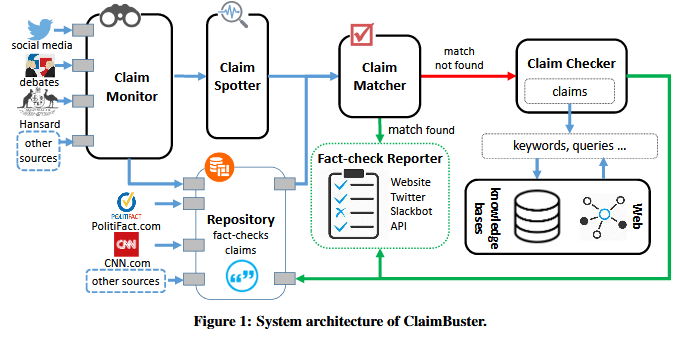
\includegraphics[width=\textwidth, draft=false]{imgs/claimbuster.PNG}
\caption{Architecture de ClaimBuster}
\label{fig1}
\end{figure}

\paragraph{ClaimMonitor}

C'est le module qui recherche les données et les récupère. Au travers de différentes sources de données il va rechercher des textes à analyser. Ce module travaille sur 3 différentes sources de données. Il y a tout d'abord la nécessité de travailler sur des informations en live afin de pouvoir instantanément évaluer les propos d'une personne : les débats politiques par exemple. C'est pour cela que les médias audiovisuels sont une importante source de données. ClaimBuster utilise différentes api pour traduire ce flux en données utilisables, notamment la structuration des données au travers de l'identification de l'orateur \cite{joseph2015speaker}. Ensuite le Claim Monitor travaille sur les données disponibles via les réseaux sociaux, il suit 2220 compte Twitter appartenant à différents type d'entité (personnalité politique, médias d'information, etc.). Seul les tweets relatifs à la politique sont gardés. Enfin ce module récupère diverses information issues de plusieurs sites web.

\paragraph{ClaimSpotter}

Une fois l'information captée et filtrée, on se retrouve avec des données liées à la politique et potentiellement constatables. Actuellement l'élément de ClaimBuster le plus mature est le Claim Spotter qui va attribuer un score à une assertion en fonction de si le fait définit est plus ou moins vérifiable : proche de 1, le fait peut être vérifié, proche de 0 le fait n'est pas vérifiable. Ce module a été construit autour d'un modèle définit par plusieurs dizaines de milliers de fait vérifiés manuellement. La précision de ce modèle est de plus de 80\%.  Le processus peut éventuellement s'arrêter à cette étape si les prochaines étapes n'apportent pas d'informations concluantes. Dans ce cas on va simplement retourner à l'utilisateur une suite de faits définis comme vérifiables et leurs scores.

Le ClaimSpotter et l'identification des faits potentiellement vérifiable s'est fait au travers du machine learning et l'apprentissage supervisé (ici on travail sur des données vérifiées). Le set de données est composé de plusieurs dizaines de milliers de phrases prononcées durant des discours, débats, etc. politiques. Chaque phrase est identifiée comme étant plus ou moins importante et plus ou moins vérifiable. PLus précisément on différencie les : 
\begin{itemize}
    \item NFS (Non Factual Sense) : qui sont des phrases banales décrivant des opinions, des traits d'humour, etc. 
    \item UFS (Unimportant Factual Sentence) : représente des phrase qui décrivent des faits qui n'ont que peu d'importance, ex : "Demain il va pleuvoir"
    \item CFS (Check-worthy Factual Sentence) : des phrases digne d'intérêts, qui valent la peine d'être vérifiées. 
\end{itemize}

Afin de noter et classifier ces phrases, ClaimBuster va utiliser des Support Vector Machines (SVM), en français, séparateurs à vaste marge. Les SVM sont une classe d'algorithmes d'apprentissage supervisée destinés à la prévision de variable qualitative binaire, c'est-à-dire des problèmes de discrimination. Plus précisément, si l'on prend une phrase de type CFS, on va la traiter comme étant positive (les autres types étant négatifs). La SVM va ensuite trouver la marge optimale et tenter de trouver un classifieur permettant de généraliser et séparer les observations et ainsi leur attribuer un score distinctif.

\paragraph{ClaimMatcher}

A partir de cette étape, on ne travail que sur des faits définis comme vérifiables, on a éliminé les opinions et tout ce qui n'est pas une assertion. Ainsi étant donné une phrase qui énonce un fait, on va essayer de prouver ou non sa véracité. Le ClaimMatcher va tenter de trouver des faits déjà vérifiés (issus de plusieurs site de fack-checking) et en rapport avec l'assertion. Pour cela il utilise 2 méthodes, l'une consiste à simplement établir une concordance entre les mots utilisés pour qualifier le fait et ceux qui définissent les faits vérifiés. L'autre se base sur une l'analyse sémantique des faits \cite{rus2013semilar}. 
\\*
Si le fait n'est pas présent, alors le système va tenter de vérifier le fait automatiquement.

\paragraph{ClaimChecker}

Le rôle de ce module est de construire un argumentaire autour du fait en collectant des informations additionnelles issues de bases de connaissances. Pour ce faire il va interroger le système de recherche de \href{https://www.wolframalpha.com/about.html}{Wolfram Alpha} grâce à des questions générées automatiquement \cite{heilman2009question}. 
\\*
Par exemple si on a l'assertion suivante : "The largest country in the world is China", et que l'on recherche ceci sur Wolfram Alpha on n'obtient aucune donnée concluante. Mais si on entre ceci : "The largest country in the world", l'assertion qui va être interprétée comme une question par l'absence de cod, le résultat retourné est la Russie. Par confrontation, on peut voir qu'il existe une différence entre les résultats et donc le fait à des chances d'être faux. Faire du fact-checking entièrement automatisé sur des questions simples est donc faisable.

Ainsi ClaimChecker va potentiellement pouvoir arriver à un verdict s'il trouve des incohérences entre les différentes questions posées. Pour assurer une fiabilité plus poussée, on envoie les questions à Google et on analyse les premiers résultats trouvés toujours pour construire un argumentaire.

\paragraph{Critique}

Le ClaimChecker va aller regarder sur les premières pages de google les choses en lien avec le fait en entrée. Comment construire un argumentaire efficace sans utiliser le TAL ? Est-ce que simplement sortir des phrases de Google sans vérifier les sources ce n'est pas tomber dans le piège de la désinformation ? Est-ce pertinent de sortir des phrases aléatoires ?

Plusieurs approches ont été utilisées pour attribuer des scores de vérifiabilité aux faits : SVM mais aussi Naive Bayes Classifier (NBC) ou encore Random Forest Classifier (RFC). SVM a été retenu du fait du haut taux de réussite (96\%, soit autant que les capacités d'analyse d'un être humain). Aucune ne se base sur le NLP, qui est ici défini comme loin d'être parfait. Mais le fait de construire son algorithme sur de l'apprentissage supervisé va rendre l'évolution de ClaimBuster bien plus compliqué. Si demain ClaimBuster souhaite étendre son activité de fact checking au-delà de la sphère politique vers tout type de domaine, ce sont des dizaines de datasets qu'il faudra construire. Même chose s'il veut s'ouvrir à d'autres langages.

Ces critiques faites, il faut quand même rappeler que le fact checking automatique n'en reste qu'à ses débuts et ClaimBuster fait parti des pionniers. Trouver un mode viable est plus important que rechercher le graal en proposant directement un système parfait. Ici le but premier est d'aider le journaliste même si la finalité serait d'obtenir un système autonome. ClaimBuster se base sur les assertions de personnalités politiques. En se perfectionnant sur cette base il pourra peut être s'ouvrir à d'autres domaines. Par exemple pour la phrase suivante : \enquote{The American Revolutionary War was a war fought between Great Britain and Russia}, ClaimBuster ne donne qu'un score de 0.32 soit un fait que l'on peut ignorer, qui n'est pas vérifiable ou ne vaut pas la peine d'être vérifié. Autre exemple : \enquote{Hayao miyazaki is dead.} ne donne qu'un score de 0.22. Mais ici ce sont des faits vérifiables et qui méritent d'être vérifiés. Pourtant Claimbuster les classe presque sur un pied d'égalité avec l'assertion suivante : \enquote{I love war} qui obtient un score de 0.17. 

Avec le TAL, il est possible d'utiliser une approche qui sera peut être au début moins viable, en effet l'outil évoluera en fonction de l'évolution du TAL. Mais cet outil sera plus simple à ouvrir à tout type de domaines et langues.

\todo{Utilisation de wikipédia pour le fact checking et plus généralement de toute base de connaissance, dans ce cas ce n'est plus orienté sur la politique mais sur quelque chose de plus vaste.}

\todo{étoffer/finir critique}

\todo{Voir les cas d'essais concrets}

\todo{Voir random forest classifier : Les Random Forest Classifier (RFC), ou forêts d'arbres décisionnels sont des techniques d'apprentissage automatique.}

\subsection{Knowledge graph}

\todo{A voir : \url{https://fr.wikipedia.org/wiki/Knowledge_Graph} : world fact book, etc.}

Un knowledge graph (ou graphe de connaissance) est défini comme une base de connaissance organisé sous forme de graphe \cite{ehrlinger2016towards} \cite{JoStichburyKG}. Comme pour une base de connaissance, l'information est organisée à l'aide d'ontologies. De part l'intégration d'une sémantique de l'information, il est possible de dériver du savoir de l'information disponible. 

\cite{dong2014knowledge}

\begin{figure}[ht]
\centering
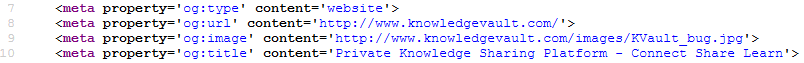
\includegraphics[width=\textwidth, draft=false]{imgs/og_example.PNG}
\caption{Exemple d'utilisation de l'open graph dans le code source d'une page : \url{http://www.knowledgevault.com/}}
\label{fig1}
\end{figure}

A lire : \url{https://nordicapis.com/automated-fact-checking-the-holy-grail-of-political-communication/}

\todo{\url{https://developers.google.com/knowledge-graph/} : permet de rechercher des infos sur des entités}

\subsubsection{Wikipédia knowledge graph}

\cite{shiralkar2017finding}

\cite{shi2016discriminative}

Le travail suivant repose sur les recherches effectuées ici \cite{ciampaglia2015computational}. Nous tâcherons d'analyser et comprendre le travail effectué, ensuite nous évaluerons sa faisabilité de son couplage avec d'autres modules qui permettront de renforcer et améliorer la fiabilité d'un système de fact checking. Suite aux recherches effectuées dans ce papier il a été prouvé qu'utiliser un graphe non orienté avec l'approche présentée ci-dessous est la plus optimale.

Pour commencer notre démonstration nous allons partir d'une assertion simple : dans un graphe une entité est liée à une autre entité s'il existe un chemin ne dépassant pas  x entités d'écart. Soit un fait en rapport avec deux entités, si ces deux entités ne sont pas liées ou si une des deux entités n'est pas présente dans le graphe, alors il y a de fortes chances pour que ce fait soit faux. Pour rappel, comme pour une base de connaissance, dans un graphe de connaissance l'information est organisée sous la forme de triplet <Sujet, Prédicat, Objet>. Entre deux entités on peut avoir plusieurs chemins de longueurs variables. Chaque chemin apporte des informations distinctes et plus ou moins précises sur la relation entre ces entités.
\\*
Par exemple pour l'assertion suivante : \enquote{Joseph Boyden wrote Three Day Road} on a 2 entités, l'écrivain et l'ouvrage. Pour arriver de l'un à l'autre on va avoir des chemins directs : l'objet livre va avoir une relation de type \enquote{auteur} qui va directement lier le livre et son auteur. On va donc attribuer une valeur forte à cette relation. Un autre chemin qui passera par des entités plus génériques se verra attribuer une importance plus faible.

\begin{figure}[H]
\centering
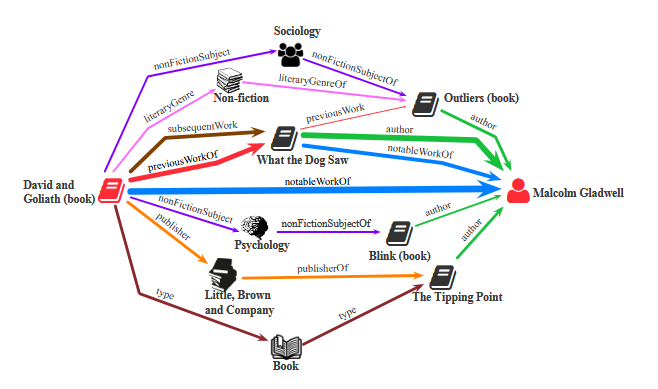
\includegraphics[width=\textwidth, draft=false]{imgs/bookAuthorKG.PNG}
\caption{Relations entre un livre et son auteur dans un graphe de connaissance \cite{shiralkar2017finding}}
\label{fig1}
\end{figure}

Dans cette approche il est important de bien définir l'impact et le rôle de la longueur du chemin entre deux entités. 
Soit G un graphe non orienté et G = (V, E) où V représente nos sommets, nos entités et E les relations entre ces entités. Pour déterminer l'existence d'un lien entre deux entités on va utiliser une opération mathématique dite \enquote{Fermeture transitive}. Le calcul de la fermeture transitive va nous permettre de créer un graphe annexe où toutes les relations sont déjà déterminées (pré-traitement qui va nous permettre de trouver plus facilement s'il existe un lien entre 2 entités) \cite{JJLGraphes}.

\begin{figure}[H]
  \centering
  \begin{minipage}[b]{0.4\textwidth}
    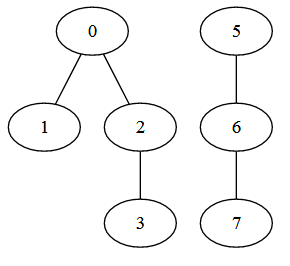
\includegraphics[width=\textwidth]{imgs/graph.PNG}
    \caption{Graphe original, non orienté}
  \end{minipage}
  \hfill
  \begin{minipage}[b]{0.4\textwidth}
    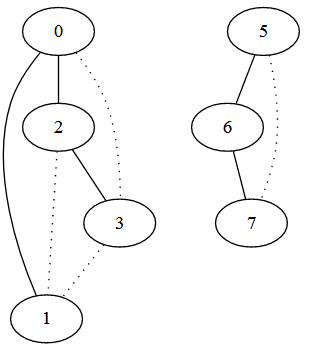
\includegraphics[width=\textwidth]{imgs/graphFT.PNG}
    \caption{Graphe et sa fermeture transitive}
  \end{minipage}
\end{figure}

\iffalse
Code du graphe (enlever les dotted pour le graphe original)

graph G {
	0 -- 1
    0 -- 2
    2 -- 3
    5 -- 6
    6 -- 7
    3 -- 1 [style=dotted]
    5 -- 7 [style=dotted]
    2 -- 1 [style=dotted]
    0 -- 3 [style=dotted]
}
\fi

On va attribuer à chaque chemin une valeur de confiance ou score de confiance qui va déterminer si ce chemin peut être utilisé pour évaluer un fait. Ce score va d'abord dépendre du degré (liens avec d'autres entités) des noeuds traversés. Une entité générique aura un degré important ce qui diminuera le score de confiance, ex : un pays, une grande organisation, etc. D'un autre côté ce score sera plus élevé s'il traverse des noeuds moins génériques, ex : personne, livre, etc. En effet un lien entre deux entités sera plus pertinent si le chemin ne traverse que des entités avec peu de relations. En suivant la même logique lorsque deux entités sont directement liées, on va leur accorder un score de confiance maximal : il n'y a pas d'intermédiaires.
\\*
Le chemin qui aura le score le plus élevé sera donc celui qui sera le plus court et qui traversera les entités les moins générique. C'est ce que l'on va appeler la proximité sémantique. Cette proximité sémantique représente le sens qui relie deux entités. Pour un fait donné, est-ce que c'est deux entités mise bout à bout ont du sens ? 

Pour le moment nous avons vu comment choisir un chemin entre deux entités, qui va nous permettre ensuite de déterminer si un fait est vrai ou faux. 

\todo{Faut-il expliquer les formules ?}

Prenons un exemple, soit des faits qui lient des villes avec des pays. Pour chaque pays et chaque villes on va tester l'assertion : \enquote{La capitale du pays x est y}.

\begin{figure}[h]
\centering
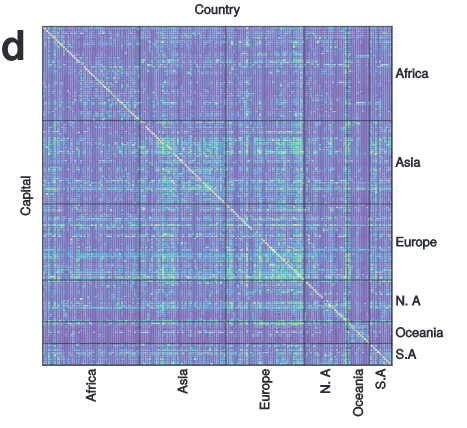
\includegraphics[draft=false, scale=0.5]{imgs/country_cap_check.PNG}
\caption{Pays et capitales groupées par continent}
\label{fig1}
\end{figure}

Plus un point est clair et plus le fait a de chance d'être vrai. Le chemin entre un pays et sa capitale possède une proximité sémantique plus forte que le chemin entre un pays et n'importe quelle autre ville. Ainsi on peut voir que cette méthode fonctionne bien, le taux de réussite enregistré est de 95\%. Cet exemple est simple mais prouve que le fact checking peut se faire au travers de graphes de connaissances. L'avantage de cette approche est qu'elle est indépendante de la langue utilisée et ne nécessite aucune technique de TAL avancée pour identifier les entités impliquées.

\paragraph{Critique} Cette méthode permet de faire du fack checking sur des faits simples. Elle se fait entre deux entités clairement définies. Le champs des possibles pour les faits à vérifier est donc limité.

\todo{A lire : https://searchengineland.com/google-researchers-introduce-system-rank-web-pages-facts-not-links-215835}

\subsubsection{Google knowledge graph}

Le Google Knowledge Graph (GKG) est ce qui permet au moteur de recherche de Google de comprendre que dans une requête il n'y a pas que des mots mais aussi des entités qui représentent des choses de la vie réelle : personne, animal, etc.

Il est possible de résumer la méthode précédente à une simple requête et à l'analyse syntaxique de la réponse. Reprenons l'assertion suivante : \enquote{Joseph Boyden wrote Three Day Road}. En annexe sont disponibles les fragments important retournés par l'api (\ref{appendix:gkg_jb}).


\subsection{Falsification d'image}

Ex : test sur donald trump qui tient la main du pape

https://www.stopfake.org/en/13-online-tools-that-help-to-verify-the-authenticity-of-a-photo/

https://arxiv.org/pdf/1801.02768.pdf : Fake Colorized Image Detection

Regarder la date d'existance de l'image sur google et la confronter avec la date de l'article.

\todo{https://www.letemps.ch/sciences/twitter-mensonge-se-diffuse-plus-vite-plus-loin-verite : Par exemple, «il y a plusieurs moyens de détecter si une image a été falsifiée», indique Ewa Kijak.}


\subsection{Vérification de la source du lien}

Baser la réputation d'un site sur son contenu au fur et à mesure des vérifications (rapport entre fake news/vraies news/news non vérifiées)

\subsection{Speaker recognition}

Ça vaut le coup de trouver un moyen de parler de la reconnaissance d'un orateur à la télé et/ou radio ?

https://ieeexplore.ieee.org/abstract/document/6853887/

\subsection{Développement prototype}

Prototype sur l'analyse de fausses images ? Plugin dans un browser ?
Construire un score de confiance.
https://wit.ai/ : NLP (pas forcément utile mais intéressant)
https://github.com/anantdgoel/HackPrincetonF16 : exemple avec pas mal d'api

\subsubsection{A faire}

\todo{credeye : \cite{popat2018credeye}}

- Parler de mon expérience dans l'analyse sémantique de texte

A rechercher : 

- Fact checking api
- Computational fact checking 

Prendre le cas de FiB et expliquer pourquoi il est mauvais ?
Voir si je ne pars pas dans trop de directions.

\clearpage


\printbibliography[
heading=bibintoc,
title={Bibliographie}
]

\clearpage

\begin{appendices}

\section{Knowledge Graph}
\subsection{Fragment du résultat retourné par le google knowledge graph pour l'entité \enquote{Joseph Boyden}}
\label{appendix:gkg_jb}

\begin{lstlisting}
{
 "@context": {
  "@vocab": "http://schema.org/",
  "goog": "http://schema.googleapis.com/",
  "EntitySearchResult": "goog:EntitySearchResult",
  "detailedDescription": "goog:detailedDescription",
  "resultScore": "goog:resultScore",
  "kg": "http://g.co/kg"
 },
 "@type": "ItemList",
 "itemListElement": [
  {
   "@type": "EntitySearchResult",
   "result": {
    "@id": "kg:/m/08gyww",
    "name": "Joseph Boyden",
    "@type": [
     "Thing",
     "Person"
    ],
    "description": "Canadian novelist",
    "image": {
     "contentUrl": "http://t2.gstatic.com/images?q=tbn:
     ANd9GcRXyYM8YrpcumM2NqJZlL5WlNncJYOgUlO-w93ztUOdOJiPK0rV",
     "url": "https://en.wikipedia.org/wiki/Joseph_Boyden"
    },
    "detailedDescription": {
     "articleBody": "Joseph Boyden CM is a Canadian novelist and short 
     story writer. His first novel, Three Day Road, won the 
     Amazon/Books in Canada First Novel Award and the Rogers Writers' 
     Trust Fiction Prize. ",
     "url": "https://en.wikipedia.org/wiki/Joseph_Boyden",
     "license": "https://en.wikipedia.org/wiki/Wikipedia:Text_of_
     Creative_Commons_Attribution-ShareAlike_3.0_Unported_License"
    }
   },
   "resultScore": 428.041321
  },
  {
   "@type": "EntitySearchResult",
   "result": {
    "@id": "kg:/m/0cwbmj",
    "name": "Three Day Road",
    "@type": [
     "Book",
     "Thing"
    ],
    "description": "Novel by Joseph Boyden",
    "detailedDescription": {
     "articleBody": "Three Day Road is the first novel from 
     Canadian writer Joseph Boyden.",
     "url": "https://en.wikipedia.org/wiki/Three_Day_Road",
     "license": "https://en.wikipedia.org/wiki/Wikipedia:Text_of_
     Creative_Commons_Attribution-ShareAlike_3.0_Unported_License"
    }
   },
   "resultScore": 13.805716
  },
  {
   "@type": "EntitySearchResult",
   "result": {
    "@id": "kg:/g/11bw4txn3g",
    "name": "Al Purdy Was Here",
    "@type": [
     "Movie",
     "Thing"
    ],
    "description": "2015 film",
    "url": "http://alpurdywashere.com/"
   },
   "resultScore": 13.146592
  }
\end{lstlisting}

\subsection{Fragment du résultat retourné par le google knowledge graph pour l'entité \enquote{Three day road}}

\begin{lstlisting}
{
 "@context": {
  "@vocab": "http://schema.org/",
  "goog": "http://schema.googleapis.com/",
  "EntitySearchResult": "goog:EntitySearchResult",
  "detailedDescription": "goog:detailedDescription",
  "resultScore": "goog:resultScore",
  "kg": "http://g.co/kg"
 },
 "@type": "ItemList",
 "itemListElement": [
  {
   "@type": "EntitySearchResult",
   "result": {
    "@id": "kg:/m/0cwbmj",
    "name": "Three Day Road",
    "@type": [
     "Book",
     "Thing"
    ],
    "description": "Novel by Joseph Boyden",
    "detailedDescription": {
     "articleBody": "Three Day Road is the first novel from 
     Canadian writer Joseph Boyden. Joseph's maternal 
     grandfather, as well as an uncle on his father's side, 
     served as soldiers during the First World War, 
     and Boyden draws upon a wealth of family narratives.",
     "url": "https://en.wikipedia.org/wiki/Three_Day_Road",
     "license": "https://en.wikipedia.org/wiki/Wikipedia:
     Text_of_Creative_Commons_Attribution-ShareAlike_3.0
     _Unported_License"
    }
   },
   "resultScore": 486.23822
  }
\end{lstlisting}

\end{appendices}

\end{document}
